\documentclass{article}
\usepackage[]{amsmath}
\usepackage[]{fullpage}
\usepackage[]{siunitx}
\usepackage[]{hyperref}
\usepackage[]{gensymb}
\usepackage{chngcntr}
\usepackage{xcolor}
\usepackage[]{graphicx}
\usepackage[]{float}
\hypersetup{
    colorlinks,
    linkcolor={blue!50!black},
    citecolor={blue!50!black}
}
\numberwithin{equation}{section}
\renewcommand{\thesection}{}
\renewcommand{\thesubsection}{}
\renewcommand{\thesubsubsection}{}
\renewcommand{\theequation}{\thesection\arabic{equation}}
\makeatletter
\def\@seccntformat#1{\csname #1ignore\expandafter\endcsname\csname the#1\endcsname\quad}
\let\sectionignore\@gobbletwo
\let\latex@numberline\numberline
\def\numberline#1{\if\relax#1\relax\else\latex@numberline{#1}\fi}
\makeatother

\title{ECE 671 Fall 2015 Assignment 3}
\author{John Rinehart}
\date{\today}


\begin{document}
\maketitle
\tableofcontents
\section*{Problem 1: Low Pass Filter Design}
\addcontentsline{toc}{section}{Problem 1: Low Pass Filter Design}

The filter designs used in this problem set follow the so-called ``insertion
loss'' design scheme. The first step in the design process is to determine the
relevant low-pass model for the filter. This low-pass model/prototype will then be used to
synthesize the appropriate filter according to some transformation rules. The
frequency may need to be transformed (since the low-pass prototype design
frequency is, by default, $\SI{1}{\radian\per\sec} $). The impedances may also
need to be transformed (since, the low-pass prototype design impedance is, by
default, $\SI{1}{\ohm}$).  

The process of selecting the low-pass prototype component values and the
low-pass prototype topology is determined by the design constraints imposed on
the designer. Typically, a pass-band is specified and an attenuation slope or
nominal attenuation at some specified frequency is chosen. This is enough to
determine the order of a particular type of filter. However, the shape of the
pass-band determines the type of filter that will, eventually, be synthesized
(equal-ripple/Chebysev or maximally flat/Butterworth). 

If the pass-band behavior and the attenuation are specified then the filter's
minimum order is specified. The choice of one of two topologies is at the hands
of the designer. The first is as shunt-first design where, in the low-pass
prototype, a capacitor shunts the generator resistance as the first reactive
element in the design. Alternatively, one can choose to place a series inductor
as the first design element in the network. As far as the low-pass prototype is
concerned, both choices are identical. It may be the case, however, that once
the impedance and frequency transformation have been completed that the
component values required would be too lossy or hard to manufacture. In this
case the alternative prototype may be selected. It is worth noting that one
prototype requires a current source and the other requires a voltage source.
This may be a design consideration as well.

Once the topology and the order are both selected it is time to select the
appropriate ``g-values'' based on the tables relevant to the filter at hand.
These g-values are the immittances (impedance or impedance or admittance) of the
corresponding low-pass prototype design. Once the topology is determined the
g-values are assigned to the capacitances and the inductances. 

The filter type specified for this design is a Butterworth/Maximally flat filter
design. The filter is to be a low-pass filter and the cut-off
(\SI{3}{\deci\bel}) frequency is specified as $ \omega_c = \SI{8}{\giga\hertz}$
and the design reference impedance is selected as \SI{50}{\ohm} . The required
required attenuation at $ \omega = \SI{13.6}{\giga\hertz}$ is \SI{16}{\deci\bel}
( $ \omega/\omega_c = 1.7 $ ). Based on tables that determine the attenuation of
different order Buttervorth filters over frequency, I will select a filter of
order five.  It's worth noting that a fourth order filter should suffice in the
case of an ideal lumped element design (it provides $\approx
\SI{18}{\deci\bel}$).  However, in case there are problems
with the implementation or in case microstrip lines do not provide as much
attenuation with varying topologies I will opt to design a fifth order filter.
The fifth order filter also has a design advantage in that the component values
are symmetrical about the middle shunt capacitor. This makes the design as
simple as designing a third order filter. But, the primary motivation is to
increase the amount of attenuation at \SI{13.6}{\giga\hertz}.

The g-values associated with this filter design are as follows:

\begin{table}[H]
    \centering
    \caption{g values}
    \label{tab:1a_g_value_table}
    \begin{tabular}{|c|c|c|c|c|c|}
        \hline $g_{1}$ & $g_{2}$  & $ g_{3} $ & $ g_{4} $ & $ g_{5} $ & $
        g_{6} $ \\ 
        \hline .618    & 1.618    & 2.0       &  1.618    & .618 & 1.0 \\
        \hline
    \end{tabular}
\end{table}

Before designing a microstrip filter, it is always good to ensure that at each
stage of the design process everything is consistent with the ideal case. So, I
will first design a lumped element filter with frequency and impedance scaling.
Assuming these values are right, I will design the microstrip model next.

In terms of the filter topology, I will choose a low-pass prototype that leads
with a shunt element (a capacitor). Based on the order of the filter and the
design topology $g_{1}, g_{3}, g_{5}$ are the low-pass prototype values for
capacitors and $g_{2}, g_{4}$ are those for inductors. $g_{6}$ is the low-pass
prototype of the 50 ohm load (termination). The following transformation
relationships will aid in taking the g-values to their appropriate component
values.

\begin{equation}
g_{N+1} Z_c \rightarrow Z_{load} \quad \quad \quad \quad
    \frac{Z_c g_n}{\omega_c} \rightarrow L \quad \quad \quad \quad
\frac{g_n}{Z_C \omega_c } \rightarrow C \nonumber
    \end{equation}

    Plugging in the appropriate values I obtain the following component values:

    \begin{table}[H]
        \centering
        \caption{Component Values}
        \label{tab:1a_comp_values}
        \begin{tabular}{|c|c|c|c|c|c|}
            \hline $C_1$ & $L_2$  & $C_3$ & $L_4$ & $C_5$ & $
            Z_{load}$ \\ 
            \hline \SI{.25}{\pico\farad}  & \SI{1.61}{\nano\henry} &
            \SI{.79}{\pico\farad}  & \SI{1.61}{\pico\farad}  &
            \SI{.25}{\pico\farad} &
            \SI{50}{\ohm}  \\
            \hline
        \end{tabular}
    \end{table}

    where N is the order of the filter (five, in this case).
    To verify the design a lumped-element model was simulated initially. The
    results and schematic are shown below. The
    attenuation was found to be $\approx \SI{-23}{\deci\bel}$ of attenuation at
    \SI{13.6}{\giga\hertz} which far exceeds the \SI{16}{\deci\bel} requirement.

    \begin{figure}[H]
        \centering
        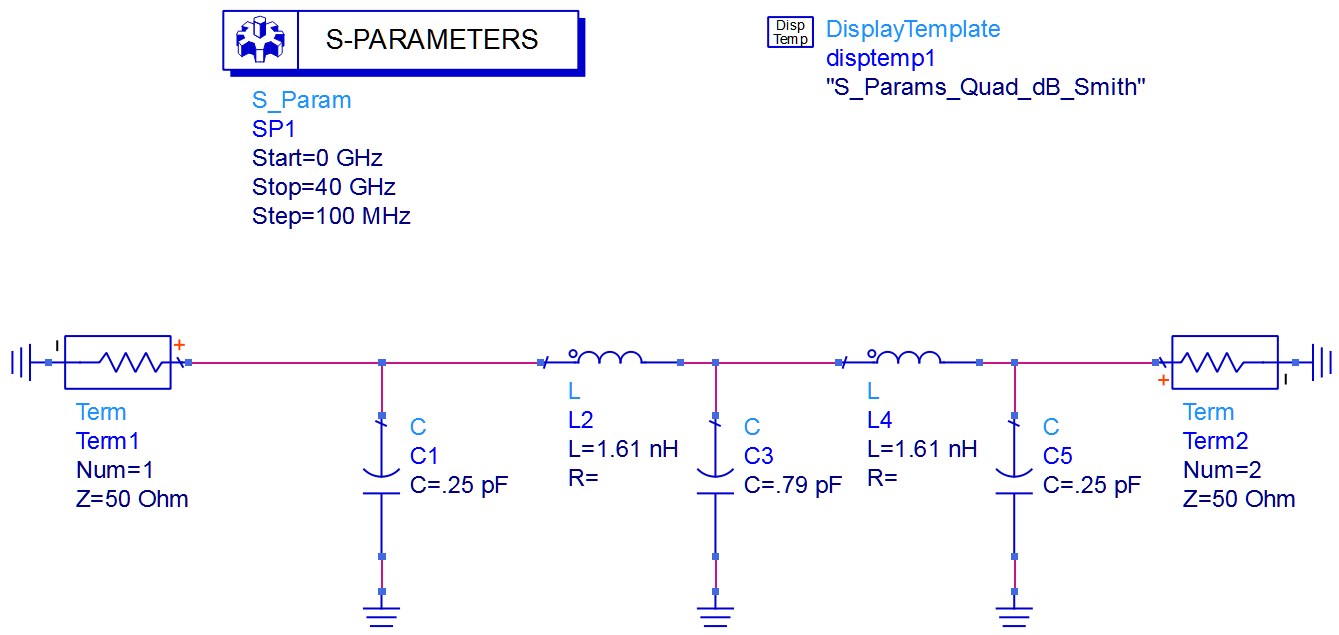
\includegraphics[width=0.8\linewidth]{img/Problem1/LumpedElementSchematic.PNG}
        \caption{Schematic for Lumped Element Low-Pass Protytpe}
        \label{fig:1a:LumpedElementSchematic}
    \end{figure}

    \begin{figure}[H]
        \centering
        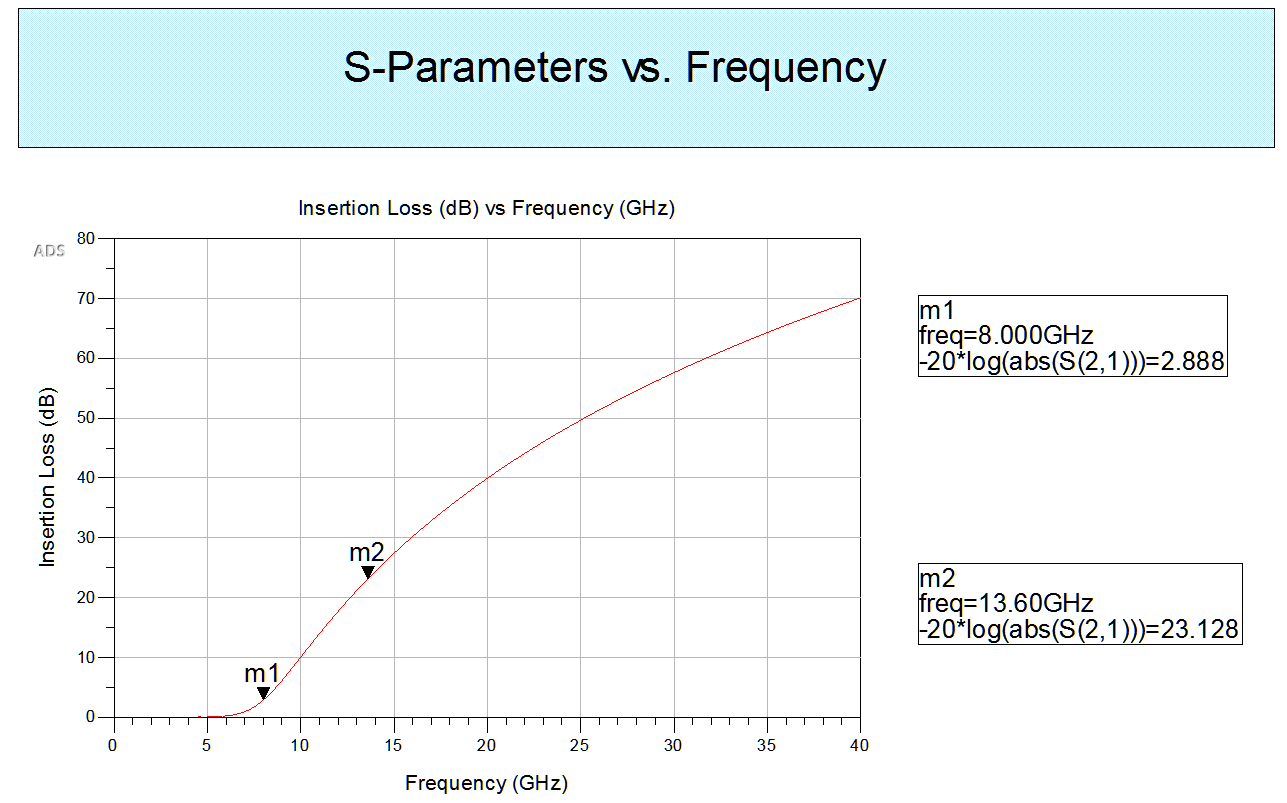
\includegraphics[width=0.8\linewidth]{img/Problem1/LumpedElementResults.PNG}
        \caption{Results of Simulating the Design in
        figure~\ref{fig:1a:LumpedElementSchematic}}
        \label{fig:imgLumpedElementResults}
    \end{figure}

    \subsection*{Problem 1a: Shunt Stub Design}
    \addcontentsline{toc}{subsection}{Problem 1a: Shunt Stub Design}

    To realize a shunt stub design I will first convert the lumped element
    capacitors into shunt stubs, directly, and use Kuroda's identity to use unit
    elements ($\lambda/8$ lengths of transmission line) to convert the series
    inductors into shunt stubs. Note that by virtue of microstrip (as well as
    the problem statement) the stubs are required to be open. Note, also, that
    the transmission line impedances needed to synthesize the open stubs will
    need to be different from \SI{50}{\ohm}, in general, in order to accommodate
    Kuroda's identity.

    In order to use Kuroda's identity I need to know the impedance of the
    various reactive elements at the design frequency. It can be shown that
    the reactance of the inductors and capacitors can be calculated as:

    \begin{align*}
        X_C^{\omega_c} = \frac{Z_c}{g_n} \quad\quad\quad\quad X_L^{\omega_c} = Z_c g_n	
    \end{align*}

    , where the reactance is calculated at the design frequency. This is the
    frequency for which we will select our transmission line stub
    impedances. Thus, constructing a table as before:

    \begin{table}[H]
        \centering
        \caption{Component Values}
        \label{tab:1a_comp_ractances}
        \begin{tabular}{|c|c|c|c|c|}
            \hline $X_{C_1}$ & $X_{L_2}$  & $X_{C_3}$ & $X_{L_4}$ & $X_{C_5}$ \\
            \hline \SI{80.9}{\ohm}  & \SI{80.9}{\ohm} & \SI{25}{\ohm}  &
            \SI{80.9}{\ohm}  & \SI{80.9}{\ohm} \\
            \hline
        \end{tabular}
    \end{table}

    In this case, the symmetry of the component values makes the design
    particularly easy. Kuroda's identity needs to be accomplished in two steps.
    First, two unit elements need to each be added to the network immediately
    following the generator and preceding the load. Then, those two unit
    elements that are ``facing the filter network'' need to each interact with
    first and last capacitor to swap the order of the reactive element and the
    transmission line. Those two capacitors, then, will become inductors. Then,
    the unit elements that have been moved to the interior of the network need
    to convert the inside inductors into capacitors. Finally, the remaining unit
    elements at the beginning and the end of the network need to turn the newly-
    fashioned inductors into capacitors. Then, the design will be completed with
    the following lumped-element topology: capacitor, unit element, capacitor,
    unit element, capacitor, unit element, capacitor, unit element, capacitor.
    To determine the appropriate microstrip transmission line impedance we need
    to convert those capacitor values to their impedance at the design
    frequency. Open stubs of length $\lambda/8$ will look like capacitors with
    impedance $Z_c$ (characteristic impedance of the transmission line used to
    synthesize the capacitor) at the design frequency, only (but sufficiently
    close to the proper capacitance over a narrow band to be useful in filter
    design).

    Doing all of this yields the following design impedances (see the appendix
    for detailed calculations):

    \begin{table}[H]
        \centering
        \caption{Open Stub Implementation}
        \label{tab:1a_open_stub_ideal}
        \begin{tabular}{|c|c|c|c|c|c|c|c|c|}
            \hline $ \text{Stub}_1 $ & $ \text{Series TL}_2 $  & $ \text{Stub}_3
            $ & $ \text{Series TL}_4 $ & $ \text{Stub}_5 $ & 
            $ \text{Series TL}_6 $ & $ \text{Stub}_7 $  & $ \text{Series TL}_8 $
                                   & $ \text{Stub}_9 $  \\
            \hline \SI{181}{\ohm} & \SI{69.7}{\ohm} & \SI{42.7}{\ohm} &
            \SI{111.8}{\ohm} & \SI{25}{\ohm} & \SI{111.8}{\ohm} &
            \SI{42.7}{\ohm} & \SI{69.4}{\ohm} & \SI{181}{\ohm} \\
            \hline
        \end{tabular}
    \end{table}
    
    Based on the design
    parameters (material and dimensions) the widths of the conductors to achieve
    these impedances are constrained. Instead of hand-calculating the impedances
    I will use line calculator tool ``LineCalc'' (bundled with ADS) to design my
    widths. In the table below I enumerate the chosen widths and lengths for the necessary
    impedance and electrical length:

    \begin{table}[H]
        \centering
        \caption{Lengths and Widths of Microstrip Sections}
        \label{tab:1a_microstrip_dimensions}
        \begin{tabular}{|c|c|c|}
            \hline Impedance ($\Omega$) & Width (mm) & Length (mm)  \\
            \hline \SI{181}{\ohm}       & .080       & 3.67         \\
            \hline \SI{69.7}{\ohm}      & 1.34       & 3.47         \\
            \hline \SI{42.7}{\ohm}      & 2.92       & 3.38         \\
            \hline \SI{111.8}{\ohm}     & .482       & 3.57         \\
            \hline \SI{25}{\ohm}        & 5.97       & 3.30         \\
            \hline
        \end{tabular}
    \end{table}

    Note that the electrical length does no change significantly with the
    characteristic impedance. This is to be expected. $\lambda/8$ at
    \SI{8}{\giga\hertz} can be found as:
    
    \[ 
        l = \frac{\lambda}{8}  = \frac{1}{8} \frac{c}{f\sqrt{\epsilon_{eff}}}
        \approx \frac{\SI{3e8}{\meter\per\second} }{8\cdot
        \SI{8e9}{\hertz}\cdot\sqrt{1.6} } \approx \SI{3.71}{mm} 
    \]
    
    where $\epsilon_{eff}$ is the effective dielectric constant which can
    usually be approximated as $\frac{\epsilon_r + 1}{2}$ for microstrip
    surrounded by air. The difference in lengths can be explained by ADS
    (LineCalc) accounting for the fringing of the different line widths and
    possibly the difference between the odd and even mode impedance for the
    different line widths. It is interesting to note that the effective length
    is smaller than would be dictated by the back-of-the-napkin calculation
    given above.

    Note also, that the larger impedance lines require much smaller widths than
    likely can be manufactured ($\sim \SI{80}{\micro\meter} $). This would be
    undesirable from a manufacturing standpoint. However, this design does not
    need to be feasible. So, it is given. The schematic and the obtained results
    follow. Noteworthy is the finiteness of the stop-band. The ideal lumped
    element model was not periodic in its response. However, transmission line
    segments have the disadvantage of having periodic frequency-domain
    responses. This is the reason for the drop in insertion loss $\approx 
    \SI{16}{\giga\hertz}$. The insertion loss can be seen to climb again
    $\approx \SI{40}{\giga\hertz}$. Note that the attenuation at
    \SI{13.6}{\giga\hertz} has climbed significantly relative to the
    lumped-element model. Apparently the stubs exhibit more rejection outside of
    the design frequency relative to the lumped elements. This is reasonable to
    expect.

    \begin{figure}[H]
        \centering
        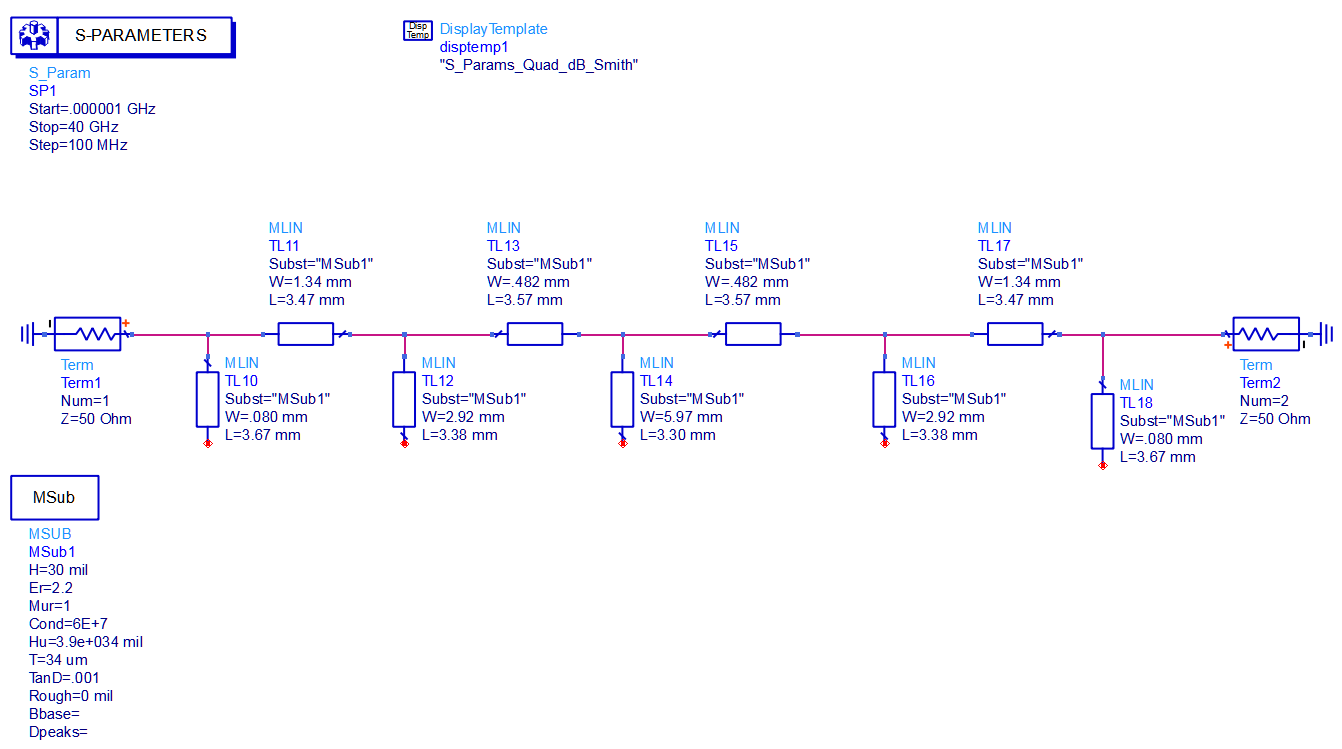
\includegraphics[width=0.8\linewidth]{img/Problem1/MicrostripStubsSchematic.PNG}
        \caption{Schematic for the Microstrip Stub Design}
        \label{fig:img/Problem1/MicrostripStubsSchematic}
    \end{figure}


    \begin{figure}[H]
        \centering
        \includegraphics[width=0.8\linewidth]{img/Problem1/MicroStripStubsResults.PNG}
        \caption{Results of Simulating the Design Shown in
        Figure~\ref{fig:img/Problem1/MicrostripStubsSchematic}}
        \label{fig:img/Problem1/MicroStripStubsResults}
    \end{figure}

    \subsection*{Problem 1b: Stepped Impedance Design}
    \addcontentsline{toc}{subsection}{Problem 1b: Stepped Impedance Design}

    The stepped impedance design is not as elegant as the previous design. To design a
    stepped impedance filter I begin using the component values for which I had
    designed my lumped element filterr. Then, I take advantage of the fact
    that short high impedance transmission line sections look like inductors and
    short section low impedance transmission line sections look like inductors.
    ``Short'' here means a small fraction of a wavelength (typically, $ < 10\%$
    of the wavelength). If the amount of time it takes the electromagnetic wave
    to propagate through the transmission line is denoted as T, the capacitance
    of a short structure looks like:

    \[ 
        C = \frac{T}{Z_c} 
    \]

    where $Z_c$ is the characteristic impedance of the line. For inductors,

    \[ 
        L =Z_c T
    \]

    These can be understood by realizing that the speed of propagation down the
    line is:

    \[ 
        v_p = \frac{1}{\sqrt{lc}} = \frac{Z_c}{l}
    \]

    Where $l$ and $c$ are the inductance and capacitance of the transmission
    line per unit length, respectively.  The propagation delay time T is related
    to $v_p$ by the distance travelled down the line $d$ as follows:

    \[ 
        T = \frac{d}{v_p} = \frac{l d}{Z_c} = \frac{L}{Z_c}
    \]

    The last inequality holds since $l d$ is just $L$, the lumped element
    equivalent inductance. Thus, to a reasonable approximation, the delay is
    expressed in terms of the characteristic impedance as given above. I have
    the lumped-element inductances and capacitances of this filter, already. I
    just have to select an appropriate delay. No impedance above \SI{130}{\ohm}
    or below \SI{10}{\ohm} can be used. Thus, I can set up the following
    inequalities for the delay in terms of the lumped elements:

    \[
        \SI{10}{\ohm} \le Z_c = \frac{T}{C} \le \SI{130}{\ohm} 
    \]

    \[ 
        \SI{10}{\ohm} \le Z_c = \frac{L}{T} \le \SI{130}{\ohm}  
    \]

    Thus, for a fixed delay, the largest capacitance will lower bound
    characteristic impedance and the largest inductance will upper bound the
    impedance, for examples. However, knowing how long the lines can be
    (assuming $d = \lambda/10$) and the speed of the wave through the medium
    (determined by $v_p = c / \sqrt{\epsilon_{eff}}$) allows me to determine T ($
    \epsilon_{eff} = \frac{\epsilon_r+1}{2} = \frac{2.2+1}{2} = 1.6$, in
    microstrip).

    \[ 
        T = \frac{\lambda/10}{v_p} = \frac{\lambda/10}{\lambda f} = 
        \frac{1}{10 f}
    \]

    For, this problem, then, $T = \SI{12.5}{\pico\second} $, since $ f =
    \SI{8}{\giga\hertz} $. Plugging this into the above expression for $C$ and
    $L$ we find the bound on $C$ and $L$ to be:

    \[ 
        \SI{96.2}{\femto\farad} \le C \le \SI{1.25}{\pico\farad} 
    \]

    \[ 
        \SI{125}{\pico\henry} \le L \le \SI{1.63}{\nano\henry}  
    \]

    Note that we meet the design requirement by the skin of our teeth. Our
    capacitances ($ C_{max} = \SI{.79}{\pico\farad} $, $ C_{min} =
    \SI{.25}{\pico\farad}  $) are well within the specification. However, the
    largest inductance is $\SI{1.61}{\nano\henry} $ which corresponds to
    \SI{129}{\ohm} and barely falls in the specification. To give the
    manufacturing some tolerance I could specify the delay to be larger. This
    would allow for larger inductances. However, this design works. Since all of
    the lengths are $\lambda/10 = \frac{c}{10 f \sqrt{1.6} } \approx
    \SI{2.96}{mm} $ all that is needed to be done is to calculated the widths of
    each section. This will be done, again, using LineCalc once the impedances
    of the lines have been determined. The estimate of the line length is
    supported by using LineCalc which gives \SI{2.73}{\milli\meter} for $Z_c =
    \SI{50}{\ohm} $. And, actually, since I'm using LineCalc to calculate the
    widths of the lines and since it seems to be determining the effective
    length of line (accounting for fringing effects, possibly) I will use
    LineCalc's values for the lengths as well. The table below enumerates the
    impedances of the lines, calculated using the above formulae:

    \begin{table}[H]
        \centering
        \caption{Line Impedance Corresponding to Lumped Elements}
        \label{tab:1b_line_impedance_of_lumped_elements}
        \begin{tabular}{|c|c|}
            \hline Component Value & Corresponding Impedance $ \Omega $ \\
            \hline $C_1 = C_5 = \SI{.25}{\pico\farad} $ &
            $\frac{\SI{12.5}{\pico\second}}{\SI{.25}{\pico\farad}} =
            \SI{50}{\ohm}$ \\
            \hline $L_1 = L_4 = \SI{1.61}{\nano\henry}$ &
            $\frac{\SI{1.61}{\nano\henry}}{\SI{12.5}{\pico\second}} \approx
            \SI{129}{\ohm}$  \\
            \hline $ C_3 =  \SI{.79}{\pico\farad} $ &
            $\frac{\SI{12.5}{\pico\second}}{\SI{.79}{\pico\farad}} \approx
            \SI{15.8}{\ohm} $ \\
            \hline
        \end{tabular}
    \end{table}

    \begin{table}[H]
        \centering
        \caption{Dimensions of Stepped Impedances}
        \label{tab:1b_stepped_impedance_dimensions}
        \begin{tabular}{|c|c|c|}
            \hline Lumped Element & Width (mm)  & Length (mm) \\
            \hline $ C_1 = C_5 $ & \SI{2.31}{mm} & \SI{2.73}{mm} \\
            \hline $ L_2 = L_4 $ & \SI{.318}{mm} & \SI{2.87}{mm}  \\
            \hline $ C_3 $ & \SI{10.4}{mm} & \SI{2.6}{mm}  \\
            \hline
        \end{tabular}
    \end{table}

    Amazingly, this filter response has $\approx \SI{6}{\deci\bel} $ of
    attenuation at $ \SI{8}{\giga\hertz} $. This is not in accordance with the
    design. I don't know why this is happening. If I am to postulate a guess,
    however, it would be that the lengths are not small enough to be considered
    ideal, thus, the capacitance of the segments is contributing a small amount
    to the inductive transmission line segments and vice versa. The way in which
    to test this would be to design at a  lower frequency such that the
    length of the lines can be constructed as smaller fractions of the
    wavelength. If the $\SI{3}{\deci\bel}$ frequency approaches the designed
    cut-off frequency then this must be the problem.
    
    The results of simulating this design follow in
    figures \ref{fig:img/Problem1/MicrostripSteppedImpedanceSchematic.PNG} and
    \ref{fig:img/Problem1/MicrostripSteppedImpedanceResults}. Note that this frequency
    response is inferior to that of the previous design.

    \begin{figure}[H]
        \centering
        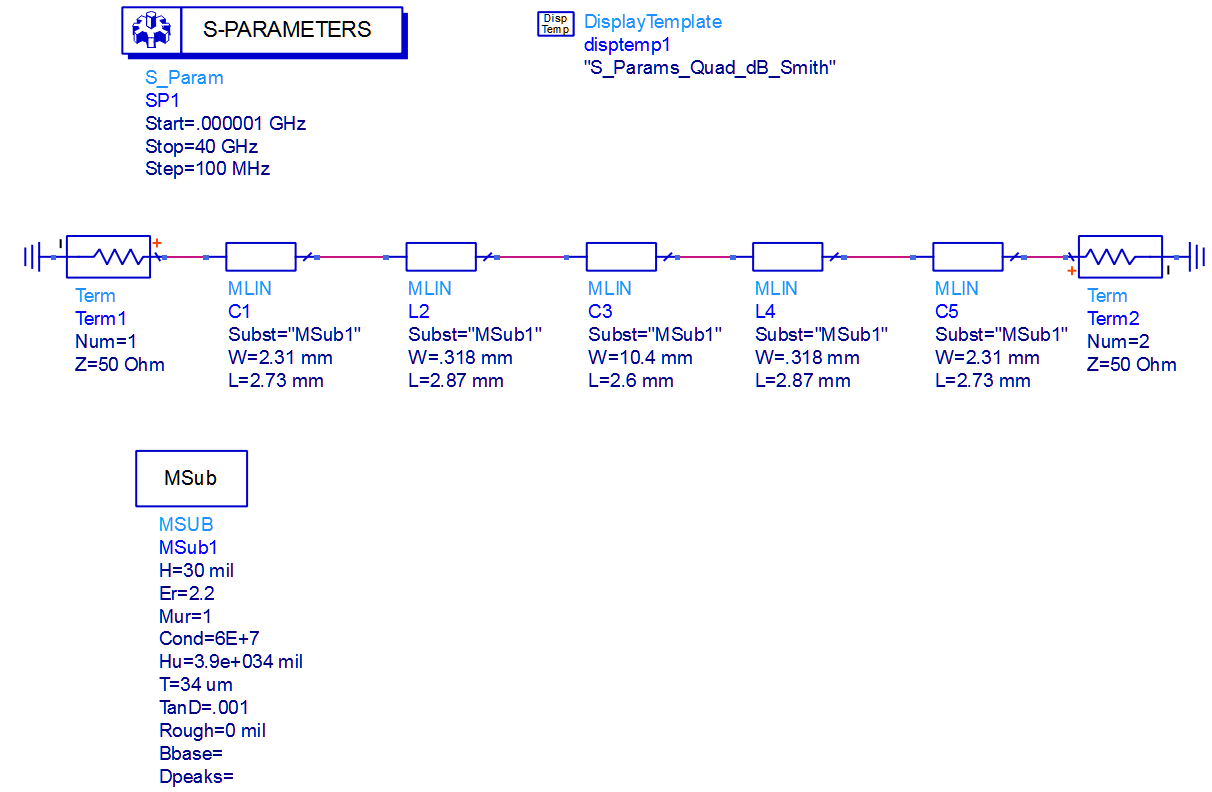
\includegraphics[width=0.8\linewidth]{img/Problem1/MicrostripSteppedImpedanceSchematic.PNG}
        \caption{Schematic for the Stepped Impedance Microstrip Design}
        \label{fig:img/Problem1/MicrostripSteppedImpedanceSchematic.PNG}
    \end{figure}

    \begin{figure}[H]
        \centering
        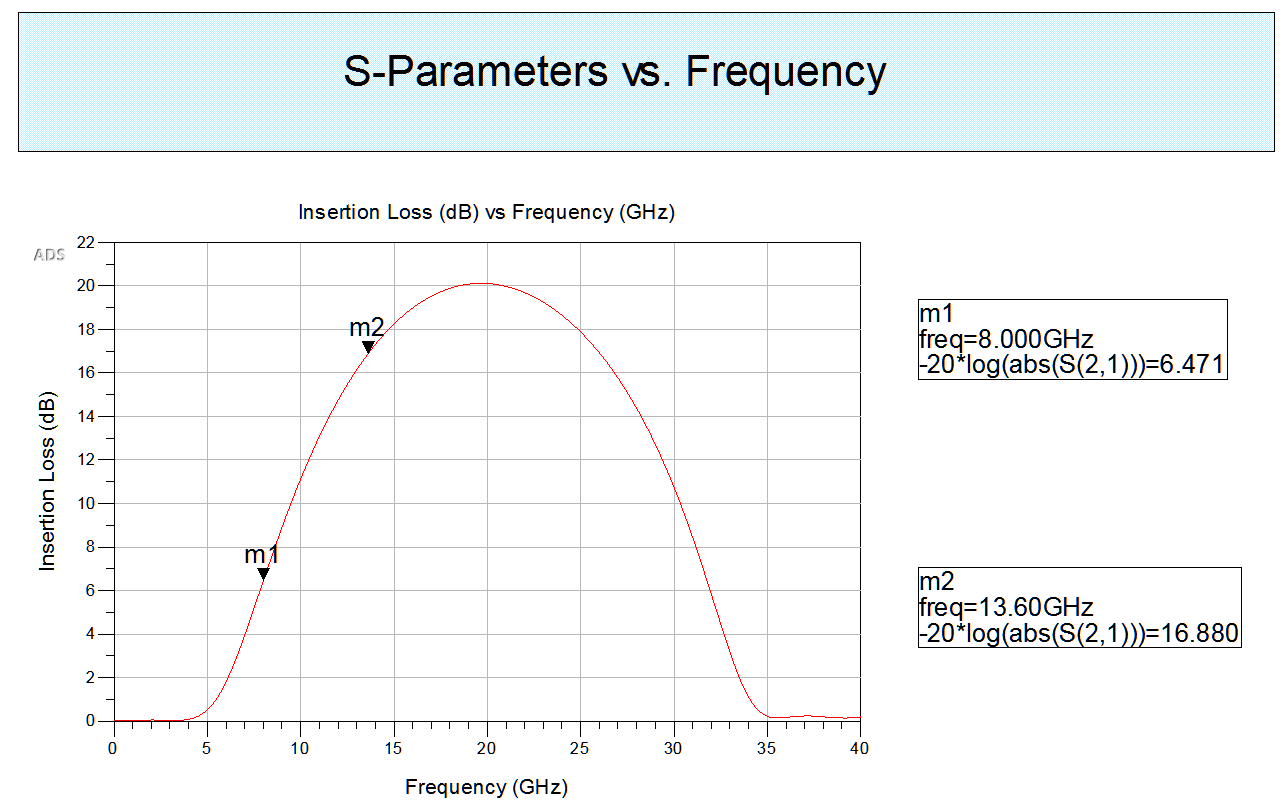
\includegraphics[width=0.8\linewidth]{img/Problem1/MicrostripSteppedImpedanceResults.PNG}
        \caption{Results for the Stepped Impedance Microstrip Design}
        \label{fig:img/Problem1/MicrostripSteppedImpedanceResults}
    \end{figure}

    \subsection*{Problem 1c: 1a and 1b with Steps and T-Junctions}
    \addcontentsline{toc}{subsection}{Problem 1c: 1a and 1b with Steps and T-Junctions}

    The last thing to do is to insert the transmission line tees into the open
    stub filter and insert the steps into the stepped impedance transmission
    line. There is nothing to change with regards to the design so I will
    include my results below in figures
    \ref{fig:img/Problem1/MicrostripStubsWithTeesSchematic} to
    \ref{fig:img/Problem1/MicrostripSteppedImpedanceWithStepsResults}. It is
    noteworthy how much different the frequency response of the stepped
    impedance differs, here, from the previous case. There are some large
    transitions in width (\SI{2.31}{mm} to \SI{.318}{mm}). Each of these
    discontinuities introduces a reflection plane that increases the amount of
    insertion loss. The fact that the insertion loss increased is not
    surprising. But, it is surprising that the insertion loss increased by as
    much as it did. Also noteworthy is how smoothed the frequency response of
    the stubs is. The maximum value of the insertion loss is much lower than it
    was before. Note that the insertion loss increased (as it did with the
    stepped impedance case) for the same reasons as given before (reflection
    plane).

    \begin{figure}[H]
        \centering
        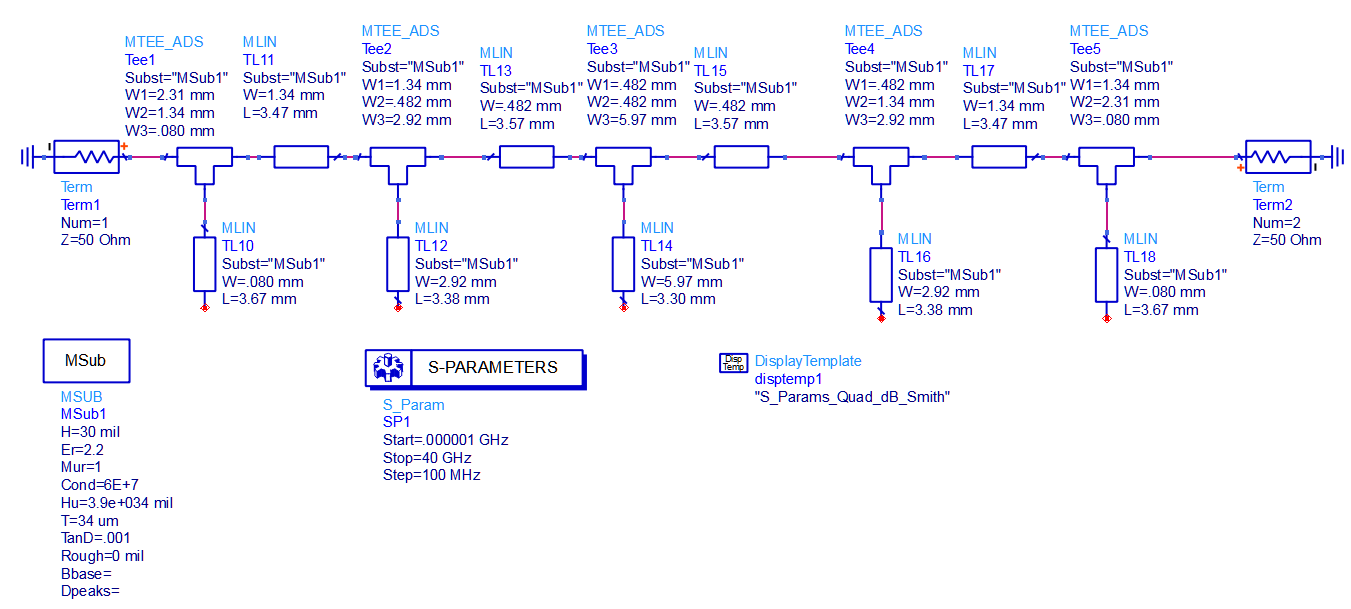
\includegraphics[width=0.8\linewidth]{img/Problem1/MicrostripStubsWithTeesSchematic.PNG}
        \caption{Schematic of Open-Stub Microstrip Design (with Tees)}
        \label{fig:img/Problem1/MicrostripStubsWithTeesSchematic}
    \end{figure}

    \begin{figure}[H]
        \centering
        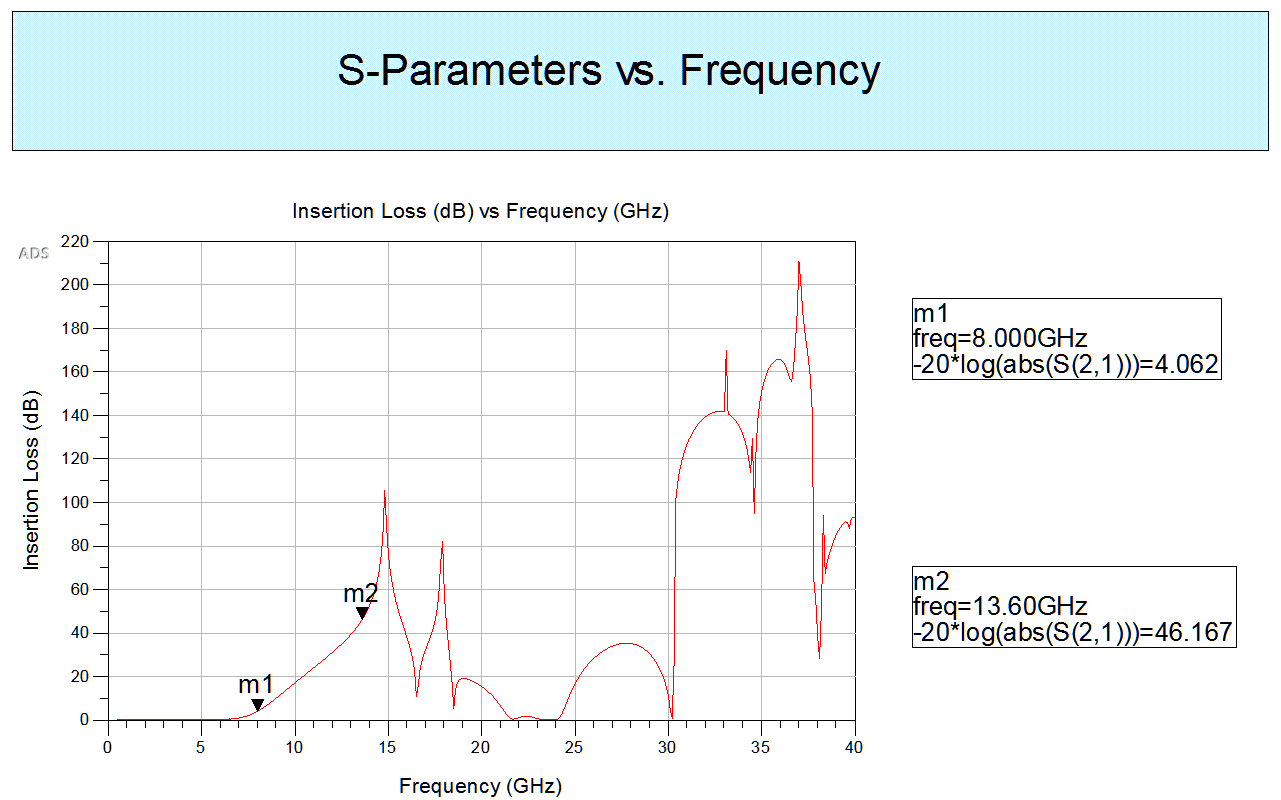
\includegraphics[width=0.8\linewidth]{img/Problem1/MicrostripStubsWithTeesResults.PNG}
        \caption{Results of Open-Stub Microstrip Design (with Tees)}
        \label{fig:img/Problem1/MicrostripStubsWithTeesResults}
    \end{figure}

    \begin{figure}[H]
        \centering
        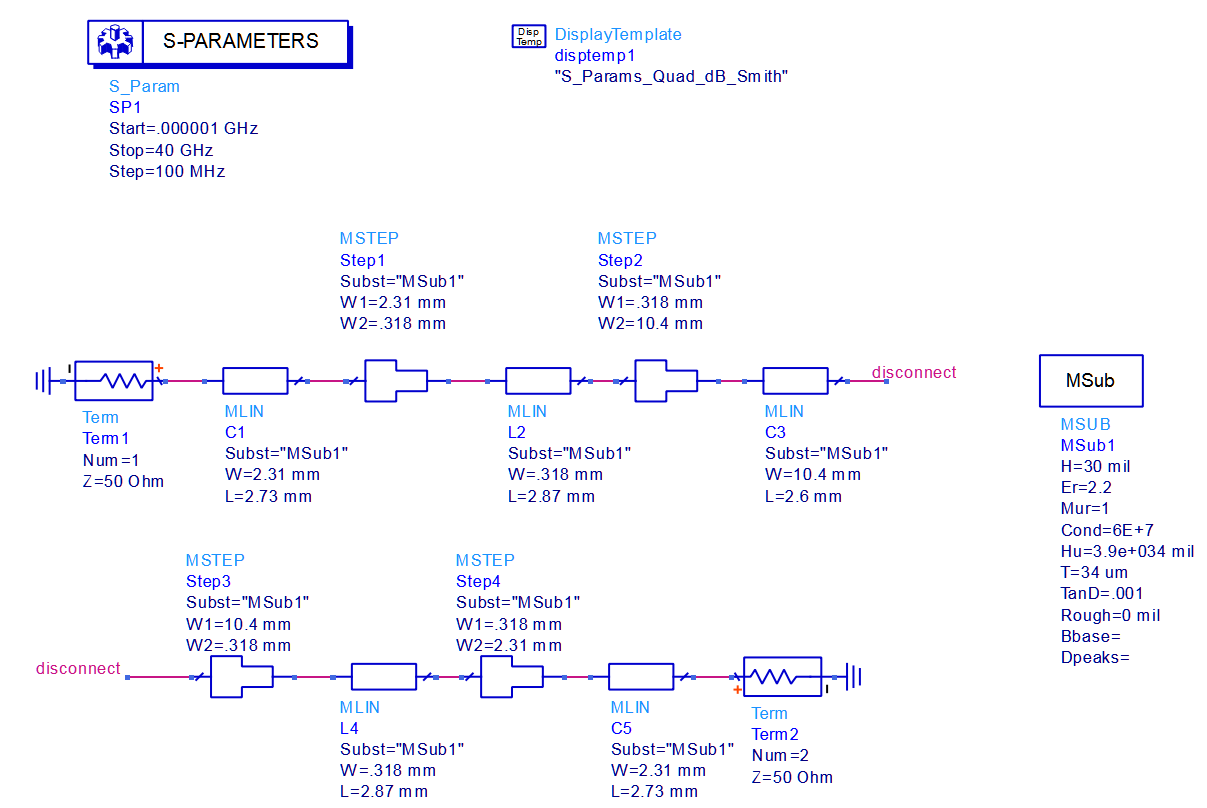
\includegraphics[width=0.8\linewidth]{img/Problem1/MicrostripSteppedImpedanceWithStepsSchematic.PNG}
        \caption{Schematic of Stepped-Impedance Microstrip (with Steps)}
        \label{fig:img/Problem1/MicrostripSteppedImpedanceWithStepsSchematic}
    \end{figure}

    \begin{figure}[H]
        \centering
        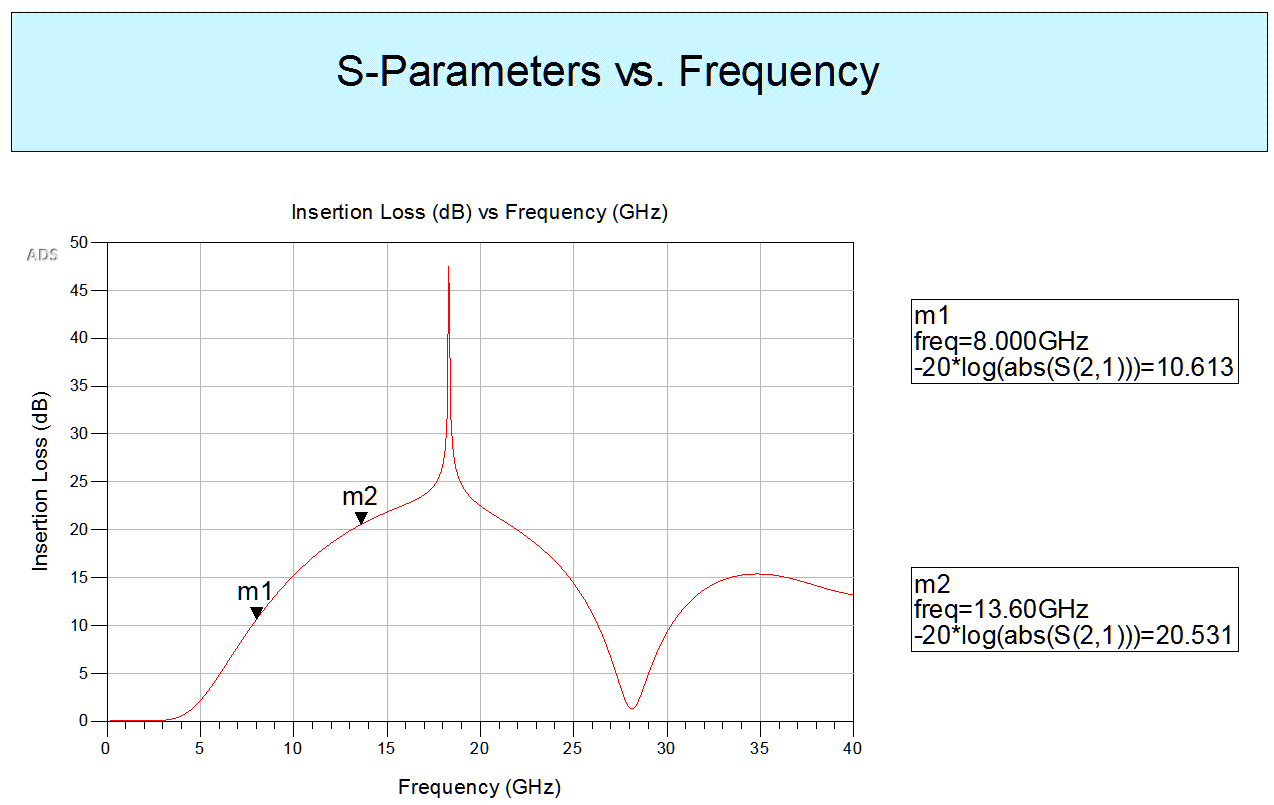
\includegraphics[width=0.8\linewidth]{img/Problem1/MicrostripSteppedImpedanceWithStepsResults.PNG}
        \caption{Results of Stepped-Impedance Microstrip (with Steps)}
        \label{fig:img/Problem1/MicrostripSteppedImpedanceWithStepsResults}
    \end{figure}

\section*{Problem 3: Equal Ripple Filter}

The first thing to do is identify the component values based on the required
order (N = 3) and the type of filter (equal ripple or Chebysev). Doing so yields:

\begin{table}[h]
    \centering
    \caption{Lumped Component Values}
    \label{tab:3a_lumped_component_values}
    \begin{tabular}{|c|c|}
        \hline $\text{g}_{\text{i}} $ & Associated $\text{g}_{\text{value}} $ \\
        \hline $ g_1 $ & 1.5963 \\
        \hline $ g_2 $ & 1.0967 \\
        \hline $ g_3 $ & 1.5963 \\
        \hline $ g_4 $ & 1.0 \\
        \hline
    \end{tabular}
\end{table}

I will choose, again, a shunt capacitor as the leading element in my low-pass
filter prototype. In transforming from the low-pass filter prototype to the
band-stop design I will need to transform the inductors into tank LC circuits
and the capacitors into series LC circuits. The resistors will simply scale with
the impedance scaling. The relevant transformations are given below:

\[ 
    C \quad \rightarrow \quad L^s = \frac{1}{\Delta \cdot C} \quad,\quad C^s = \frac{\Delta
    \cdot C}{\omega_0^2}
\]

where the superscript ``s'' denotes a series LC element and $\Delta = \omega_2
- \omega_1$ (the stop-band bandwidth), $\omega_0 = \sqrt{\omega_1\omega_2}$ is
the geometric mean of the stop-band bandwidth. Similarly for the inductor
transformation we have:

\[ 
L \quad \rightarrow \quad C^t = \frac{1}{\Delta \cdot L} \quad,\quad L^t = \frac{\Delta
\cdot L}{\omega_0^2}
\]

where the same definitions as previously defined for the capacitor hold. In this
case, we know the fractional bandwidth is $10 \%$ and that the center frequency
(the midpoint of the two endpoints of the stop-band $\omega_1$ and $\omega_2$)
is \SI{3}{\giga\hertz}. Thus, we \textbf{could} construct the following two relationships:

\[
    \omega_{center} = \frac{\omega_1 + \omega_2}{2} \quad,\quad
    \text{BW}_{\text{frac}} = \frac{\omega_2 - \omega_1}{\omega_{center}}
\]

We have been given $\text{BW}_{\text{frac}}$ and $\omega_{center}$. This allows
us to solve for $\omega_1$, $\omega_2$ and $\omega_0$. However, the above
definition for the center frequency is not typically what is used. Instead, the
geometric mean of $\omega_1$ and $\omega_2$ (which is $\omega_0$) is what is
defined as the center frequency of the band-stop filter. Thus, $\omega_0 =
\SI{3}{\giga\hertz}$. So, we actually have the following two equations:

\[ 
    \omega_{center} = \omega_0 = \sqrt{\omega_1 \omega_2} \quad,\quad
    \text{BW}_{\text{frac}} = \frac{\Delta}{\omega_0} = \frac{\omega_2 -
    \omega_1}{\omega_0}
\]

Solving the above equations for $\omega_1$ and $ \omega_2 $ yields:

\[ 
    \omega_1 \approx \SI{2.85}{\giga\hertz} \quad,\quad \omega_2 \approx
    \SI{3.15}{\giga\hertz} 
\]

Now, in the chosen topology, $g_1, g_3$ represent capacitors and $g_2$
represents an inductor. I will start by transforming the capacitors. First,
though, I will obtain the capacitance and inductance after impedance scaling.
The reference impedance for this problem is \SI{75}{\ohm}. Thus, the capacitor
and inductor values are as follows:

\begin{table}[h]
    \centering
    \caption{Component Values after Impedance Scaling}
    \label{tab:2_comp_values}
    \begin{tabular}{|c|c|}
    \hline $ C_1 = C_3$ & \SI{21.2}{\milli\farad} \\
    \hline $ L_2 $ & \SI{82.3}{\henry} \\
    \hline
    \end{tabular}
\end{table}

Determining the series LC elements:

\begin{table}[h]
    \centering
    \caption{Series LC elements after Band-Stop Transformation}
    \label{tab:2_series_elements}
    \begin{tabular}{|c|c|}
        \hline L & \SI{25.0}{\nano\henry} \\
        \hline C & \SI{112}{\femto\farad} \\
        \hline
    \end{tabular}
\end{table}

Doing the same thing for the inductor transformation:

\begin{table}[h]
    \centering
    \caption{Tank LC Elements after Band-Stop Transformation}
    \label{tab:2_tank_elements}
    \begin{tabular}{|c|c|}
    \hline L & \SI{437}{\pico\henry} \\
    \hline C & \SI{6.45}{\pico\farad} \\
    \hline
    \end{tabular}
\end{table}

Now, I just need to make the elements lossy. The capacitors are to have a
quality factor of 40 and the inductors are to have a quality factor of 20.
Assuming a series-lossy model for the inductor and a shunt-lossy model for the
capacitor we have the following relationships between Q, R, and the element
values:

\[ 
    R^L_s = \frac{X^L_s}{Q^L_s} \quad,\quad R^C_p = X^C_p Q^C_p
\]

where the superscript denotes the element type and the subscript denotes
whether the resistor is in parallel (p) or in series (s) with the inductor (L)
or capacitor (C). We can now solve for the four resistances for the four
elements:

\begin{table}[h]
    \centering
    \caption{Resistance of Each of the Imperfect Lumped Elements}
    \label{tab:lumped_element_resistance}
    \begin{tabular}{|c|c|}
        \hline $R_L$~\text{(series LC)} & $\frac{\omega_c L}{Q_L} \approx
        \SI{23.6}{\ohm}$ \\
        \hline $R_C$~\text{(series LC)} & $ \frac{Q_C}{\omega_c C}\approx
        \SI{18.9}{\kilo\ohm} $ \\
        \hline $R_L$~\text{(tank LC)} & $\frac{\omega_c L}{Q_L} \approx
        \SI{412}{\milli\ohm}$ \\
        \hline $R_C$~\text{(tank LC)} & $ \frac{Q_C}{\omega_c C}\approx
        \SI{329}{\ohm} $ \\
        \hline
    \end{tabular}
\end{table}

Inserting the above resistances into the design and simulating yields a much
lower attenuation over the stop-band. The bandwidth doesn't change significantly,
which is surprising since the peak flattens a lot. But, the \SI{3}{\deci\bel}
points are at almost the exact same frequencies.

\section*{Problem 3: 90 \degree Hybrid Junction with Tee}
\addcontentsline{toc}{section}{Problem 3: 90 \degree Hybrid Junction with Tee}

\subsection*{Problem 3a: Deriving Some Result}
\addcontentsline{toc}{subsection}{Problem 3a: Deriving Some Result}

This problem was pretty fun to solve. The first thing to realize is that the
system is matched everywhere (despite the potential difference in the transmission line
lengths at the tee). The impedance looking into just the tee (not cascaded with
the hybrid junction) is $\frac{\left( Z_0/\sqrt{2} \right)^2}{Z_{L}}$, where
$Z_L$ is the equivalent impedance of the two branches in the tee ($Z_L =
\frac{Z_0}{2}$). This means the input impedance to the tee is $Z_0$. The 90
\degree hybrid junction is matched by design. Thus, the cascade of these two
devices is matched. Now, the hybrid tee will propagate some input voltage
$V_{in}$ in the following way: At the end of one end of the branch (the one of
length a) the following voltage will appear:

\[ 
    V_a = \frac{V_{in}}{2} e^{-j \beta a} 
\]

At the end of the other branch (of length b-a) will appear the other voltage:

\[ 
    V_{b-a} = \frac{V_{in}}{2} e^{-j \beta \left( b-a \right)} 
\]

Now, the voltage appearing at port 2 because of the voltages at ports 1 and 4
($V_{b-a}$ and $V_a$, respectively) is:

\[ 
    V_2 = \frac{-1}{\sqrt{2}} \left( j V_a + V_{b-a}  \right) 
\]

Similarly, the voltage appearing at port 3 because of the voltages at ports 1
and 4 is:

\[ 
    V_3 = \frac{-1}{\sqrt{2}} \left( j V_{b-a} +  V_{a} \right)
\]

This can be seen by inspecting the scattering parameters of the 90 \degree
hybrid coupler:

\[ 
    S_{90\degree} = -\frac{j}{\sqrt{2}} \begin{pmatrix}
        0 & 1 & -j & 0 \\ 1 & 0 & 0 & -j \\ -j & 0 & 0 & 1 \\ 0 & -j & 1 & 0
    \end{pmatrix} 
\]

Now, the power coming out of port 2 is $\frac{|V_2|^2}{Z_0}$ and similarly with
the port coming out of port 3. Thus:

\[ 
    \frac{P_3}{P_2} = \frac{\left| V_3 \right|^2}{\left| V_2 \right|^2} 
\]

The prefactors in front of $V_2$ and $V_3$ can evidently be dropped (since they
are the same). This leaves the following expression to be evaluated:

\[
    \frac{P_3}{P_2} = \frac{\left| jV_{b-a} + V_a \right|^2}{\left| j V_a +
    V_{b-a} \right|^2} = \frac{\left| V_a \right|^2 + \left| V_{b-a} \right|^2 +
    jV_{b-a} V_a^* - j V_{b-a}^*V_a }{\left| V_a \right|^2 + \left| V_{b-a} \right|^2 +
j V_a V_{b-a}^* -j V_a^* V_{b-a}}
\]

But, $\left| V_a \right| = \left| V_{b-a} \right| = \frac{V_{in}}{2}$. In fact,
$V_{in}^2$ will show up in each term in the numerator and the denominator. Thus,
the new expression for the power ratio can be written as:

\begin{align*}
\frac{P_3}{P_2} =& \frac{2 + 2\Re ( j V_{b-a}V_a^*)}{2 + 2\Re ( j V_a V_{b-a}^* )} \\
    =& \frac{1+\Re \left( e^{j\pi/2}e^{-j\beta
    a}e^{j\beta\left(b-a\right)}\right)}
    {1+\Re\left(e^{j \pi/2} e^{j \beta a} e^{-j \beta \left( b-a \right)}
    \right)} \\
    =& \frac{1 + \cos \left( \pi/2 - \beta a + \beta \left( b-a \right)
    \right)}{1 + \cos \left( \pi/2 + \beta a -\beta\left(b-a\right)\right)} \\
    =& \frac{1+\cos \left( \pi/2 + \beta b - 2\beta a \right)}
    {1 + \cos \left( \pi/2 -\beta b + 2 \beta a \right)} \\
    \intertext{But, $\beta = 2\pi/\lambda$ and $b = \lambda/4$ so that $\beta b
    = \pi/2$}
    =& \frac{1+\cos\left(\pi-2\beta a \right)}{1+\cos\left(2\beta a \right)} \\
    =& \frac{1-\sin(2\beta a)}{1+\cos \left( 2\beta a \right)} \\
    =& \frac{\sin^2(\beta a)}{\cos^2( \beta a )} \\
    =& \tan^2(\beta a)\
    \intertext{But, $\beta = \pi/(2 b)$. So, finally:} \\
    =& \tan^2(\frac{\pi a}{2 b})
\end{align*}

\subsection*{Problem 3b: Designing a 1/3, 2/3 power splitter}
\addcontentsline{toc}{subsection}{Problem 3a: Deriving Some Result}

By tuning the dimension a until the power coming out of port 3 is half of that
coming out of port 2 we will have a 1/3, 2/3 power splitter. 1/3 of the input
power at port 1 will exit port 3. The remaining 2/3 will exit port 2. In order
to accomplish this we require that:

\begin{align*}
    \frac{P_3}{P_2} = \frac{1}{2} =& \tan^2 \left( \frac{\pi a}{2 b} \right) \\
    \frac{1}{\sqrt{2}} =& \tan \left( \frac{\pi a }{2 b} \right) \\
    \intertext{This is a trigonometric function which will exhibit periodic
        solutions. I will choose the solution that minimizes the angle
    (minimizing the ratio of $a:b$).} \\
    \arctan \left( \frac{1}{\sqrt{2}} \right) \frac{2}{\pi} =& \frac{a}{b}
    \approx \SI{392}{\milli\radian} \\
    a \approx .392 b
\end{align*}

The problem asks me to design a power divider. This previous work, then, is just
one step. I still need to select an operation frequency and pick the lengths of
the transmission lines. I won't design a microstrip circuit since the problem
does not explicitly ask for it. I will assume an ideal transmission line model.
I need to select a length $b$. I will assume that $b = \lambda/4$ so that the
electrical length of that line is $45 \degree$. This constrains a to be $\approx
35.3 \degree$ long.  I will assume an operation frequency of
\SI{1}{\giga\hertz}. The electrical lengths of the branch-line hybrid are $\beta
\lambda/4 = 45 \degree$. The topology of the quadrature hybrid coupler are given
in the course notes. Note that $\frac{50}{\sqrt{2}}\approx 35.355$. From this I
obtain the schematic  and results shown in figures
\ref{fig:img/Problem3/PowerSplitterSchematic.PNG} to
\ref{fig:img/Problem3/PowerSplitterInputReturnLoss.PNG}. 

Note that the design criterion (that of 1/3, 2/3 power split) is attained nearly
exactly. At \SI{1}{\giga\hertz} $S_{3,1} \approx \SI{-4.76}{\deci\bel}$ and
$S_{2,1} \approx \SI{-1.77}{\deci\bel}$, which correspond to power transfer
ratios of $\approx .334$ and $\approx .666$, respectively. That's what you get
for using ideal components. It's strange that it's not exactly right. A large
part of the error is likely due to rounding in these hand calculations.

\begin{figure}[H]
    \centering
    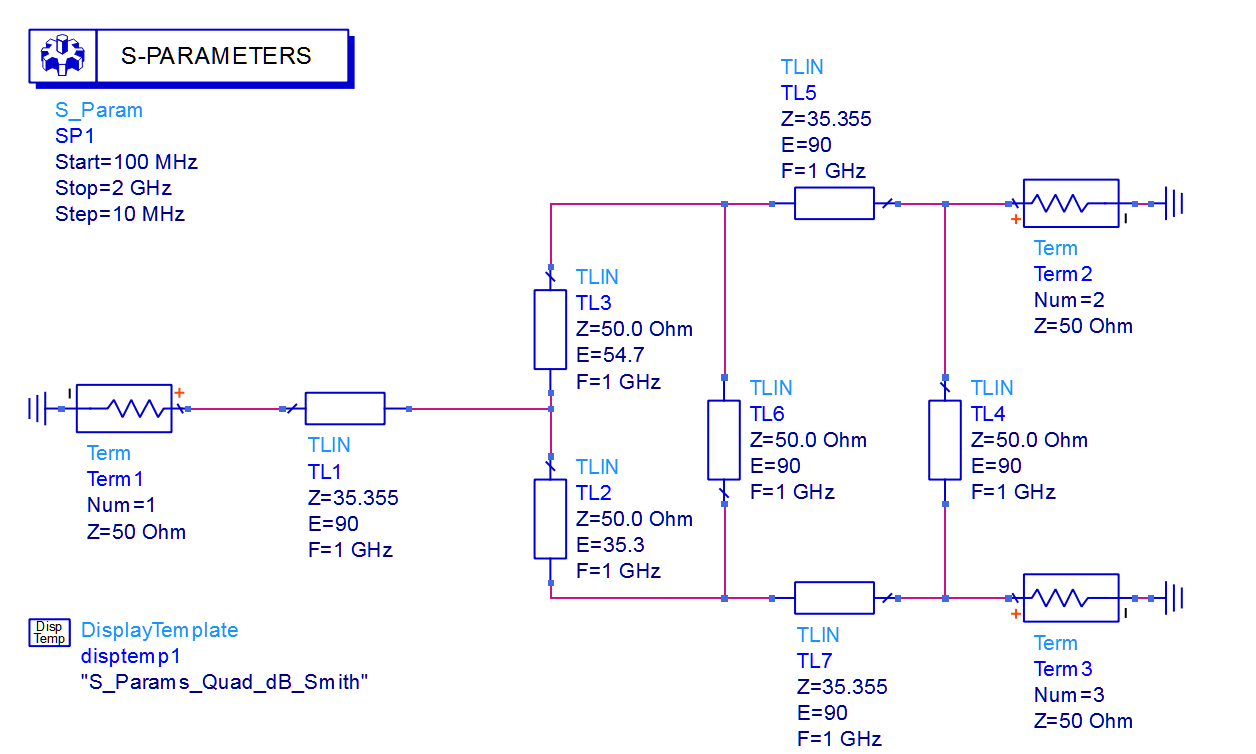
\includegraphics[width=0.8\linewidth]{img/Problem3/PowerSplitterSchematic.PNG}
    \caption{Schematic of the Designed Power Splitter}
    \label{fig:img/Problem3/PowerSplitterSchematic.PNG}
\end{figure}

\begin{figure}[H]
    \centering
    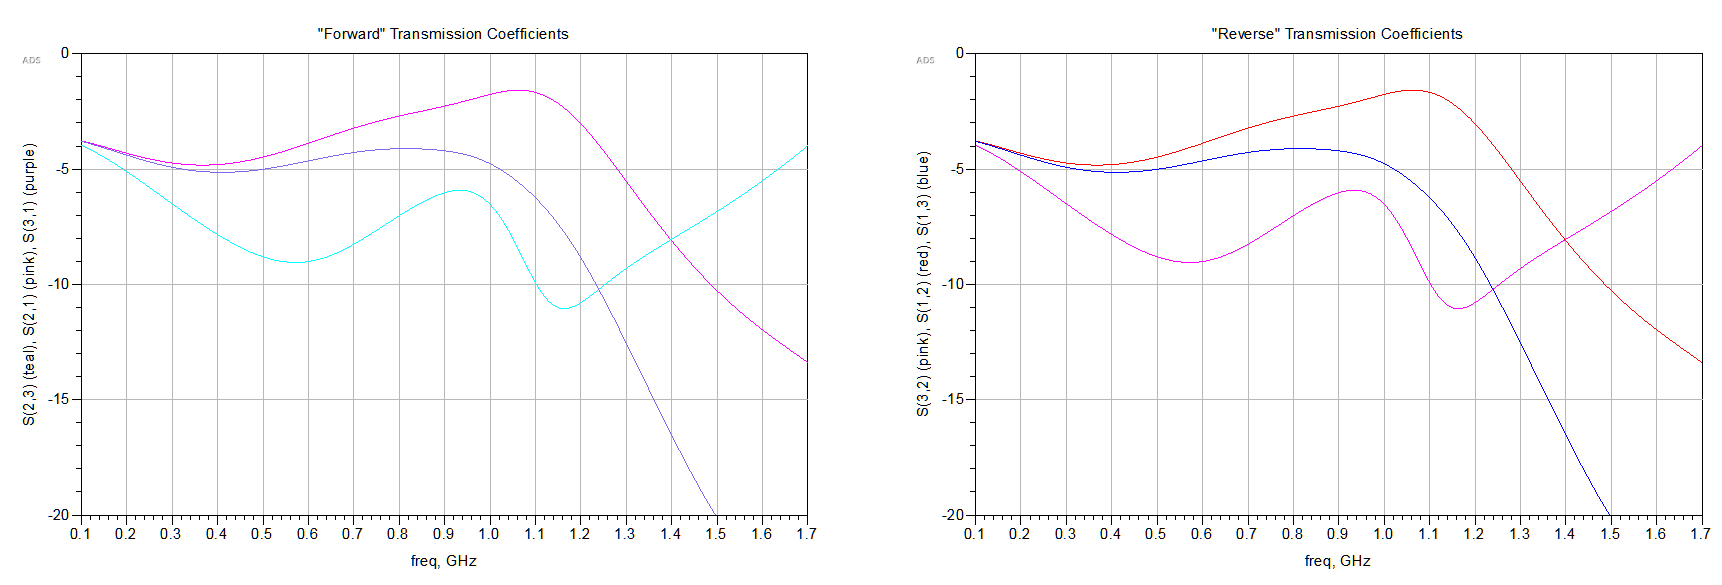
\includegraphics[width=0.8\linewidth]{img/Problem3/PowerSplitterTransmissionCoefficients.PNG}
    \caption{Transmission Coefficients for the Designed Power Splitter}
    \label{fig:img/Problem3/PowerSplitterTransmissionCoefficients}
\end{figure}

\begin{figure}[H]
    \centering
    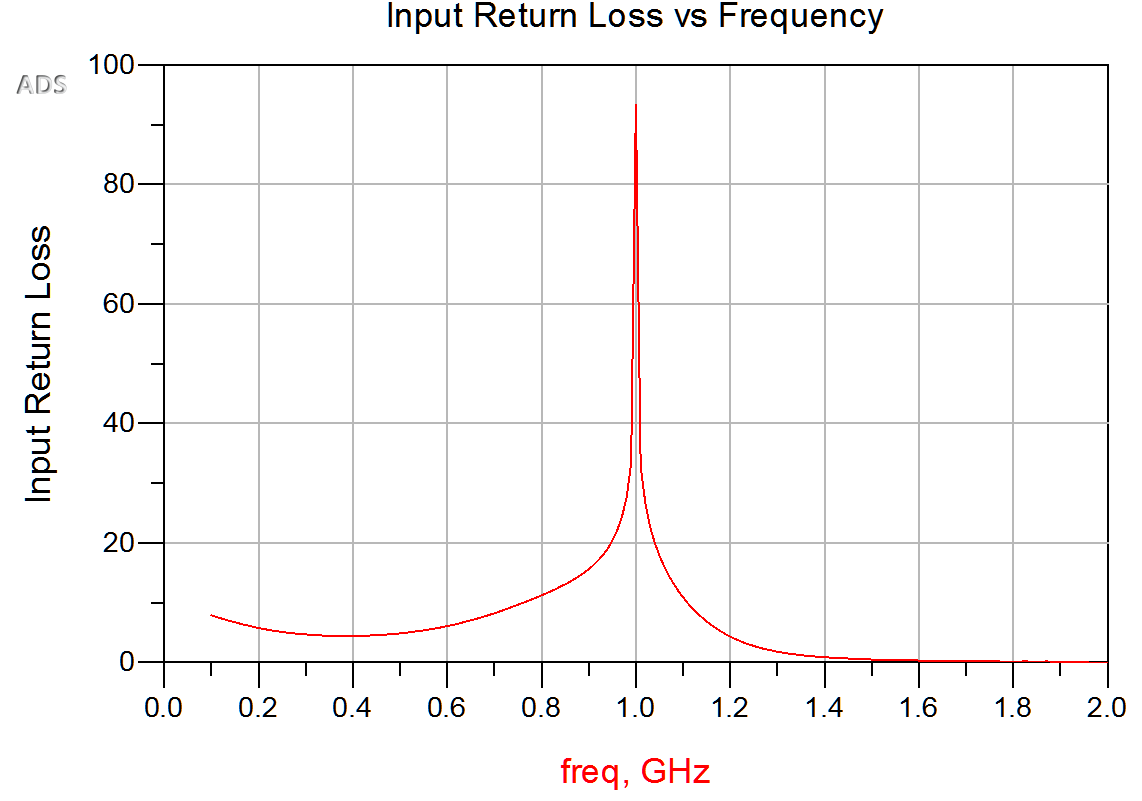
\includegraphics[width=0.8\linewidth]{img/Problem3/PowerSplitterInputReturnLoss.PNG}
    \caption{Input Return Loss for the Designed Power Splitter}
    \label{fig:img/Problem3/PowerSplitterInputReturnLoss.PNG}
\end{figure}

\section*{Problem 4: A Better Circulator}
\addcontentsline{toc}{section}{Problem 4: A Better Circulator}

The scattering parameter matrix is given in the following form:

\[ 
    S_{circ} = \begin{pmatrix}
        0 & a & b \\ b & 0 & a \\ a & b & 0
    \end{pmatrix} 
\]

where $ a = .03$ and $b = .93$. This problem will be broken up into different
stages considering the different paths the wave will follow. First, the
incident wave $V_{in}$ will encounter the first circulator. Because $S_{3,1}$ is
nonzero, some of the wave ( $V_3 = a V_{in}$ ) will head down towards a second
circulator. This wave will travel into the first port of that circulator and out
of the second port $V_{RF_3} = a b V_{in}$. The wave that traveled out of the
second port of the first circulator will travel towards its second circulator.
Some of that wave will travel through port three of the rightmost circulator
$V_{RF_5} = b a V_{in}$. Now, we have to consider exactly how both waves
interact at ports 2 and 3 to combine to give the wave at port 4 ($V_{RF_7}$).

The ideal 180\degree~coupler has the following scattering parameters:

\[
    S_{180 \degree} = \frac{-j}{\sqrt{2}} \begin{pmatrix}
        0 & 1 & 1 & 0 \\ 1 & 0 & 0 & -1 \\ 1 & 0 & 0 & 1 \\ 0 & -1 & 1 & 0
    \end{pmatrix}
\]

Thus, the wave incident at port 2 will contribute to a wave at port 4 that is
180\degree~out of phase with respect to that incident wave. The wave at port 3
will give rise to a wave at port 4 that is in phase with that incident wave.
Thus:

\[ 
    V_{RF_7} = -V_{RF_3} + V_{RF_5} = -a b V_{in} + a b V_{in} = 0
\]

Thus, even though the circulator is not ideal, the three-port device formed by all of
these devices is ideal. However, it's worth noting that this result assumes the
rat race coupler is ideal (balanced) such that the waves perfectly cancel.
Practically, this will not occur and the non-idealities of the circulator have
to be compared to the non-idealities of the rat race coupler.

\begin{figure}[H]
    \centering
    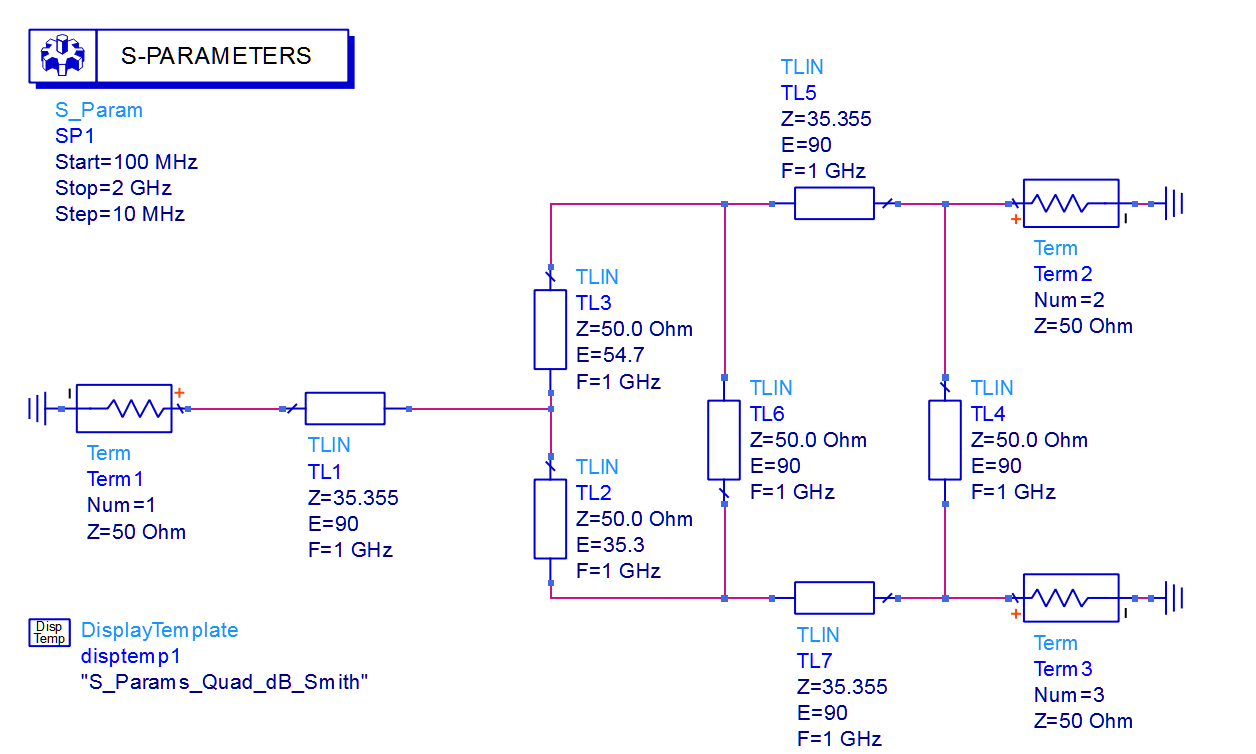
\includegraphics[width=0.8\linewidth]{img/Problem3/PowerSplitterSchematic.PNG}
    \caption{Schematic for the Power Splitter}
    \label{fig:img/Problem3/PowerSplitterSchematic}
\end{figure}

\end{document}
